Building upon the validated homography matrix and the continuously interpolated 2D tracking data, the final objective of the pipeline is to reconstruct the bowling ball's trajectory in real-world dimensions. As shown in Figure \ref{fig:2d_trajectory}, the interpolated trajectory is first visually rendered as a continuous trace directly onto the perspective video feed. Simultaneously, these continuous pixel coordinates are multiplied by the homography matrix to project the ball's positional path onto a two-dimensional bird's-eye view. It is important to note that, for graphical visualization purposes, the rendered top-down lane shown on the right side of the figure is intentionally distorted, compressed longitudinally and expanded laterally compared to true physical proportions. While the underlying homographic projection calculates metrically accurate spatial coordinates, mapping the projected trajectory onto this visually scaled lane significantly improves readability, exaggerating the transverse dynamics to make the ball's lateral hook clearly perceptible to the viewer.

\begin{figure}[htbp]
    \centering
    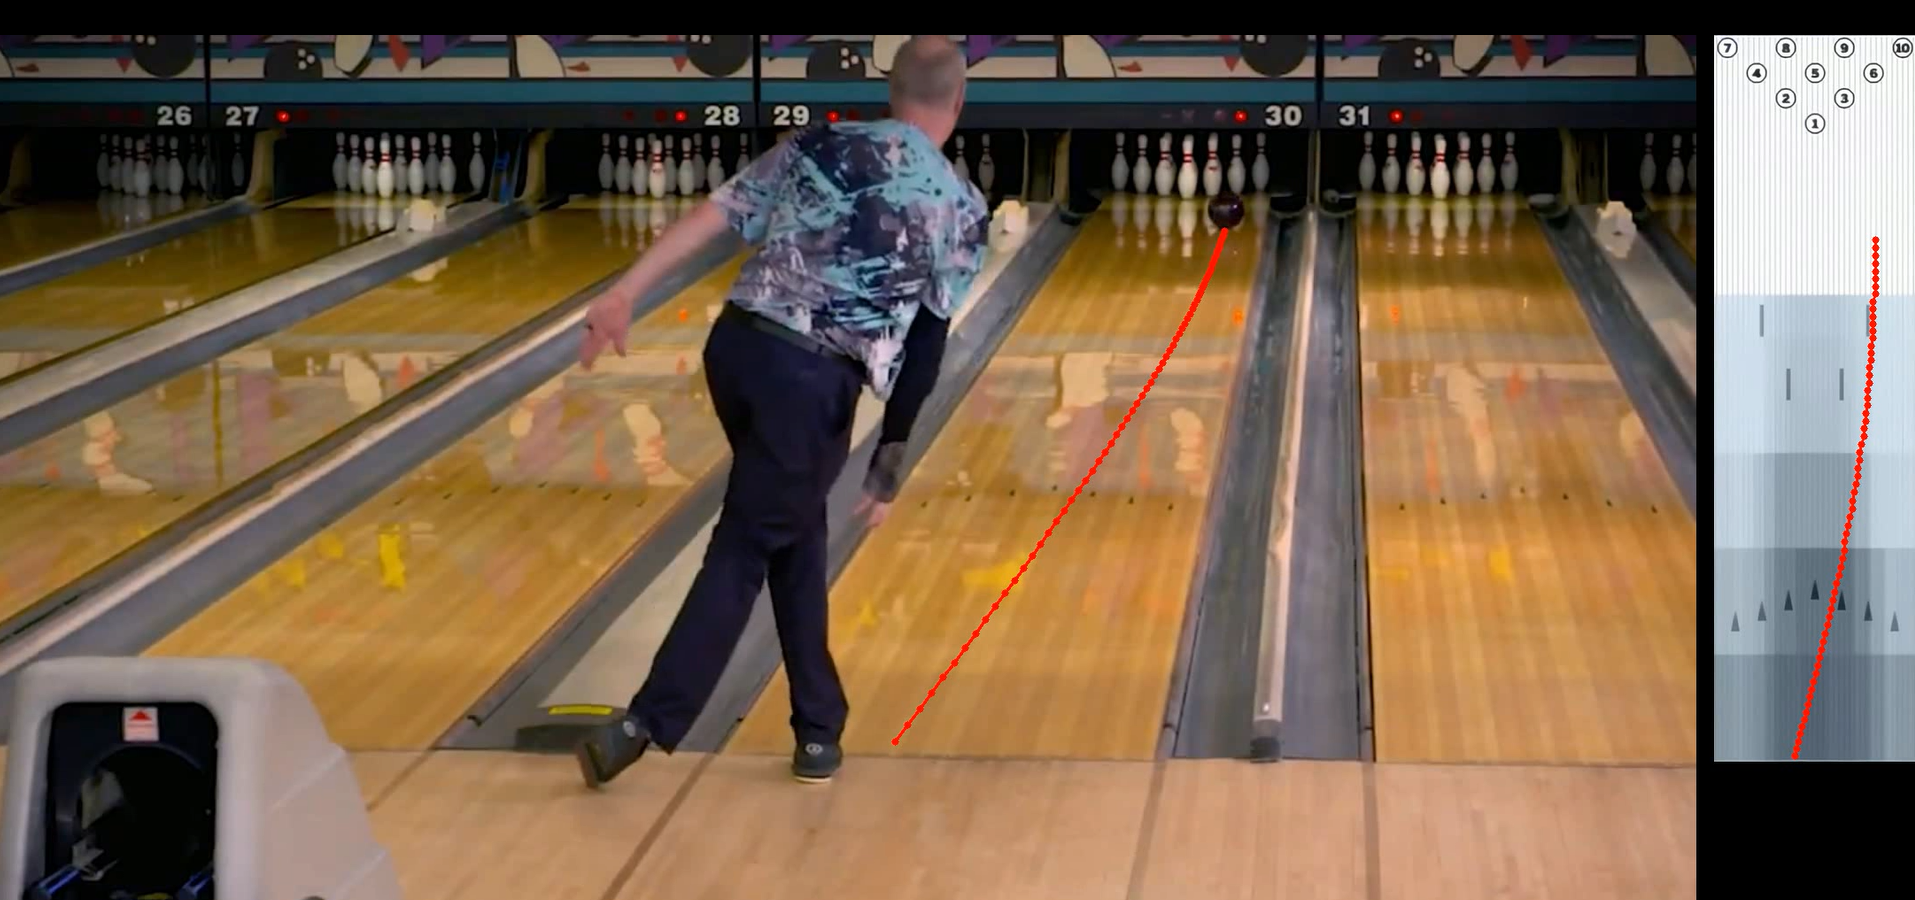
\includegraphics[width=0.9\textwidth]{figures/results/final_visualization_clip2.png}
    \caption{2D Trajectory mapping. Left: The interpolated tracking data is traced in red on the original perspective image plane. Right: The pixel coordinates are warped via the computed homography matrix into a normalized bird's-eye view. The graphical representation of the lane is intentionally scaled to exaggerate transverse movement, revealing the true lateral curvature of the throw.}
    \label{fig:2d_trajectory}
\end{figure}

To provide a comprehensive spatial analysis, this metrically accurate 2D planar data is subsequently extended into a full three-dimensional physical representation. The pipeline defines a real-world coordinate system anchored at the bottom-left corner of the physical lane (the origin), with the X and Y axes corresponding to the standardized physical length and width of the playing surface. The Z axis elevates the physical radius of the bowling ball above the floor plane, allowing for a volumetric representation of the movement.

Qualitative analysis of the final spatial visualizations (see Figure \ref{fig:3d_reconstruction}) confirms the success of the end-to-end pipeline. The reconstructed trajectory exhibits a smooth curvature that accurately mirrors the ball's hook dynamics from the original video. Ultimately, this proper spatial alignment demonstrates that the integrated computer vision pipeline successfully translates raw 2D pixel data into a reliable 3D kinematic model.

% \begin{figure}[htbp]
%     \centering
%     
\includegraphics[width=0.75\textwidth]{figures/results/clip2_3d_1.png}
    
%     \vspace{0.2cm}
    
%     
\includegraphics[width=0.75\textwidth]{figures/results/clip2_3d_2.png}
    
%     \vspace{0.2cm}
    
%     
\includegraphics[width=0.75\textwidth]{figures/results/clip2_3d_3.png}
    
%     \caption{Three-dimensional spatial reconstruction of the lane and ball trajectory. The 2D homographic data is mapped into a physical coordinate space, rendering the lane's true dimensions, the origin point, and a volumetric model of the ball following the calculated trajectory path. Top to bottom: sequential shifts in viewing perspective highlight the spatial relationship between the origin and the trajectory curve.}
%     \label{fig:3d_reconstruction}
% \end{figure}

\begin{figure}[htbp]
    \centering
    % Top Row: First viewing angle
    
\includegraphics[width=0.75\textwidth]{figures/results/clip2_3d_1.png}
    
    \vspace{0.4cm}
    
    % Middle Row: Second viewing angle (Left) with the separated legend (Right)
    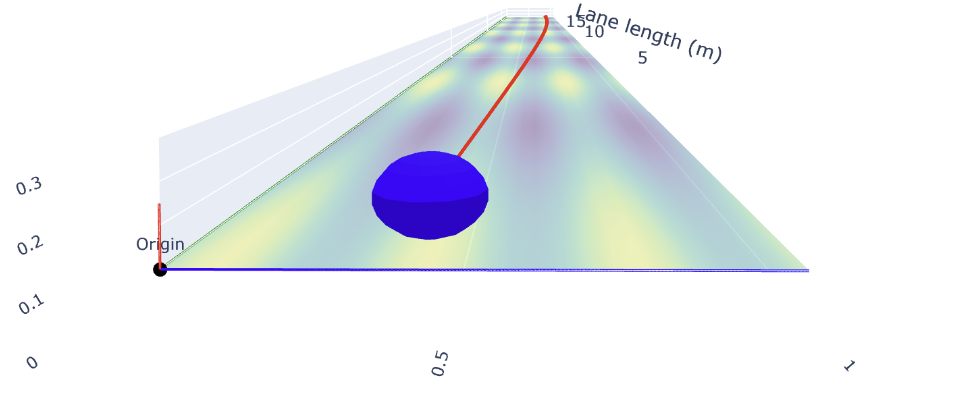
\includegraphics[width=0.75\textwidth]{figures/results/clip2_3d_2_1.png}
    \hfill
    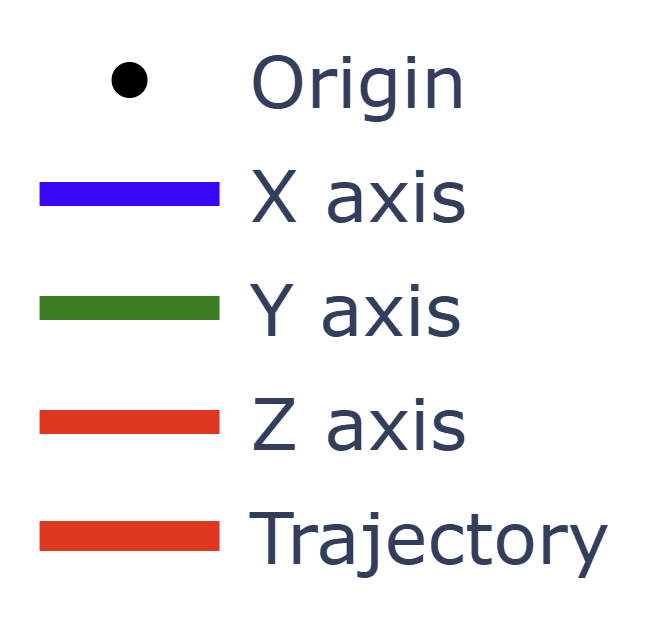
\includegraphics[width=0.20\textwidth]{figures/results/clip2_3d_1_2.png}
    
    \vspace{0.4cm}
    
    % Bottom Row: Third viewing angle
    
\includegraphics[width=0.75\textwidth]{figures/results/clip2_3d_3.png}
    
    \caption{Three-dimensional spatial reconstruction of the lane and ball trajectory, shown from three distinct viewing perspectives to better illustrate the 3D spatial mapping.}
    \label{fig:3d_reconstruction}
\end{figure}